\chapter{Attacks}

We present four novel attacks against the \eos system. The \NODEDOS
(\S\ref{label_reentrancy-attack}) attack undermines service availability of \BPs,
thus contributing to block generation delays in the \eos system.
%
The \TESER (\S\ref{label_teser}) and \SCPDOS (\S\ref{SCPDOS}) attacks deplete the
resources staked for the execution of \SCs, including \cpu and \ram, thus
resulting in the denial of \SC services.
%
The \TOCTOU (\S\ref{label_toctou}) attack exploits the controversial \EOS design
decision that allows \SC updates. The adversary starts by obtaining the
sensitive permission with her benign \SC code and then changes it later to
deplete the \ram of the victims. The adversary may then ask a ransom for
releasing victims' \ram.
%
We emphasize that all the presented attacks harness attack vectors unique to
\eos.

In this section, we describe each attack and demonstrate its feasibility with an
attack experiment that measures its potential impact on \PLATFORM.
%

\PP{Experimental setup.}
We conducted experiments to measure how much loss each attack can cause in
\PLATFORM. We used a machine running 64-bit Ubuntu 16.04.3 LTS with Intel Core
i7-8700 CPU at 3.20 GHz (12 cores), 32 GB of RAM, and 200 GB SSD.
%
For the testing environment, we prepared two different versions of \eos on the
machine: version 1.1.1, where we discovered the \NODEDOS attack, and version
1.7.3, which is the latest stable version to confirm the patch for the \NODEDOS
attack and to test the feasibility of other attacks.
%
Each version of \eos is initialized with default system SCs that manage the
resources of \eos and the execution of other SCP-provided SCs.
%
Note that we have never conducted the presented attacks against the actual \eos
system in production for ethical and respectable research.

\PP{Collected SCs.}
We collected 3,212 \SCs from 3,600 accounts in the \eos main network
and installed them in our testing environment.





\section{Block delay attack}
\label{label_reentrancy-attack}
The \NODEDOS attack causes a delay in the production of blocks in a \BP by
generating an unacceptable number of spurious transactions. These spurious
transactions elicit misbehaviors in the \BP when scheduling them, thus usurping
opportunities that should have been used for processing valid transactions.
This entails huge financial losses for participants in \PLATFORM by delaying
the transactions that require immediate completion.
%
We note that this attack targets all \SCs running in \BPs, not a
particular \SC, which makes the attack even more critical.

A DoS on any blockchain system is indeed a critical security threat, as many
emerging blockchain systems strive to provide a high-availability service with
a high TPS.
%
Because the \eos system only depends 21 representative \BPs to process worldwide transactions, the DoS on a single \BP may cause a significant TPS degradation.
%
We first describe the \eos block generation procedures and then explain how
the \NODEDOS attack exploits the procedures.



\begin{figure}[!t] %%%% t->h or ht
\centering
  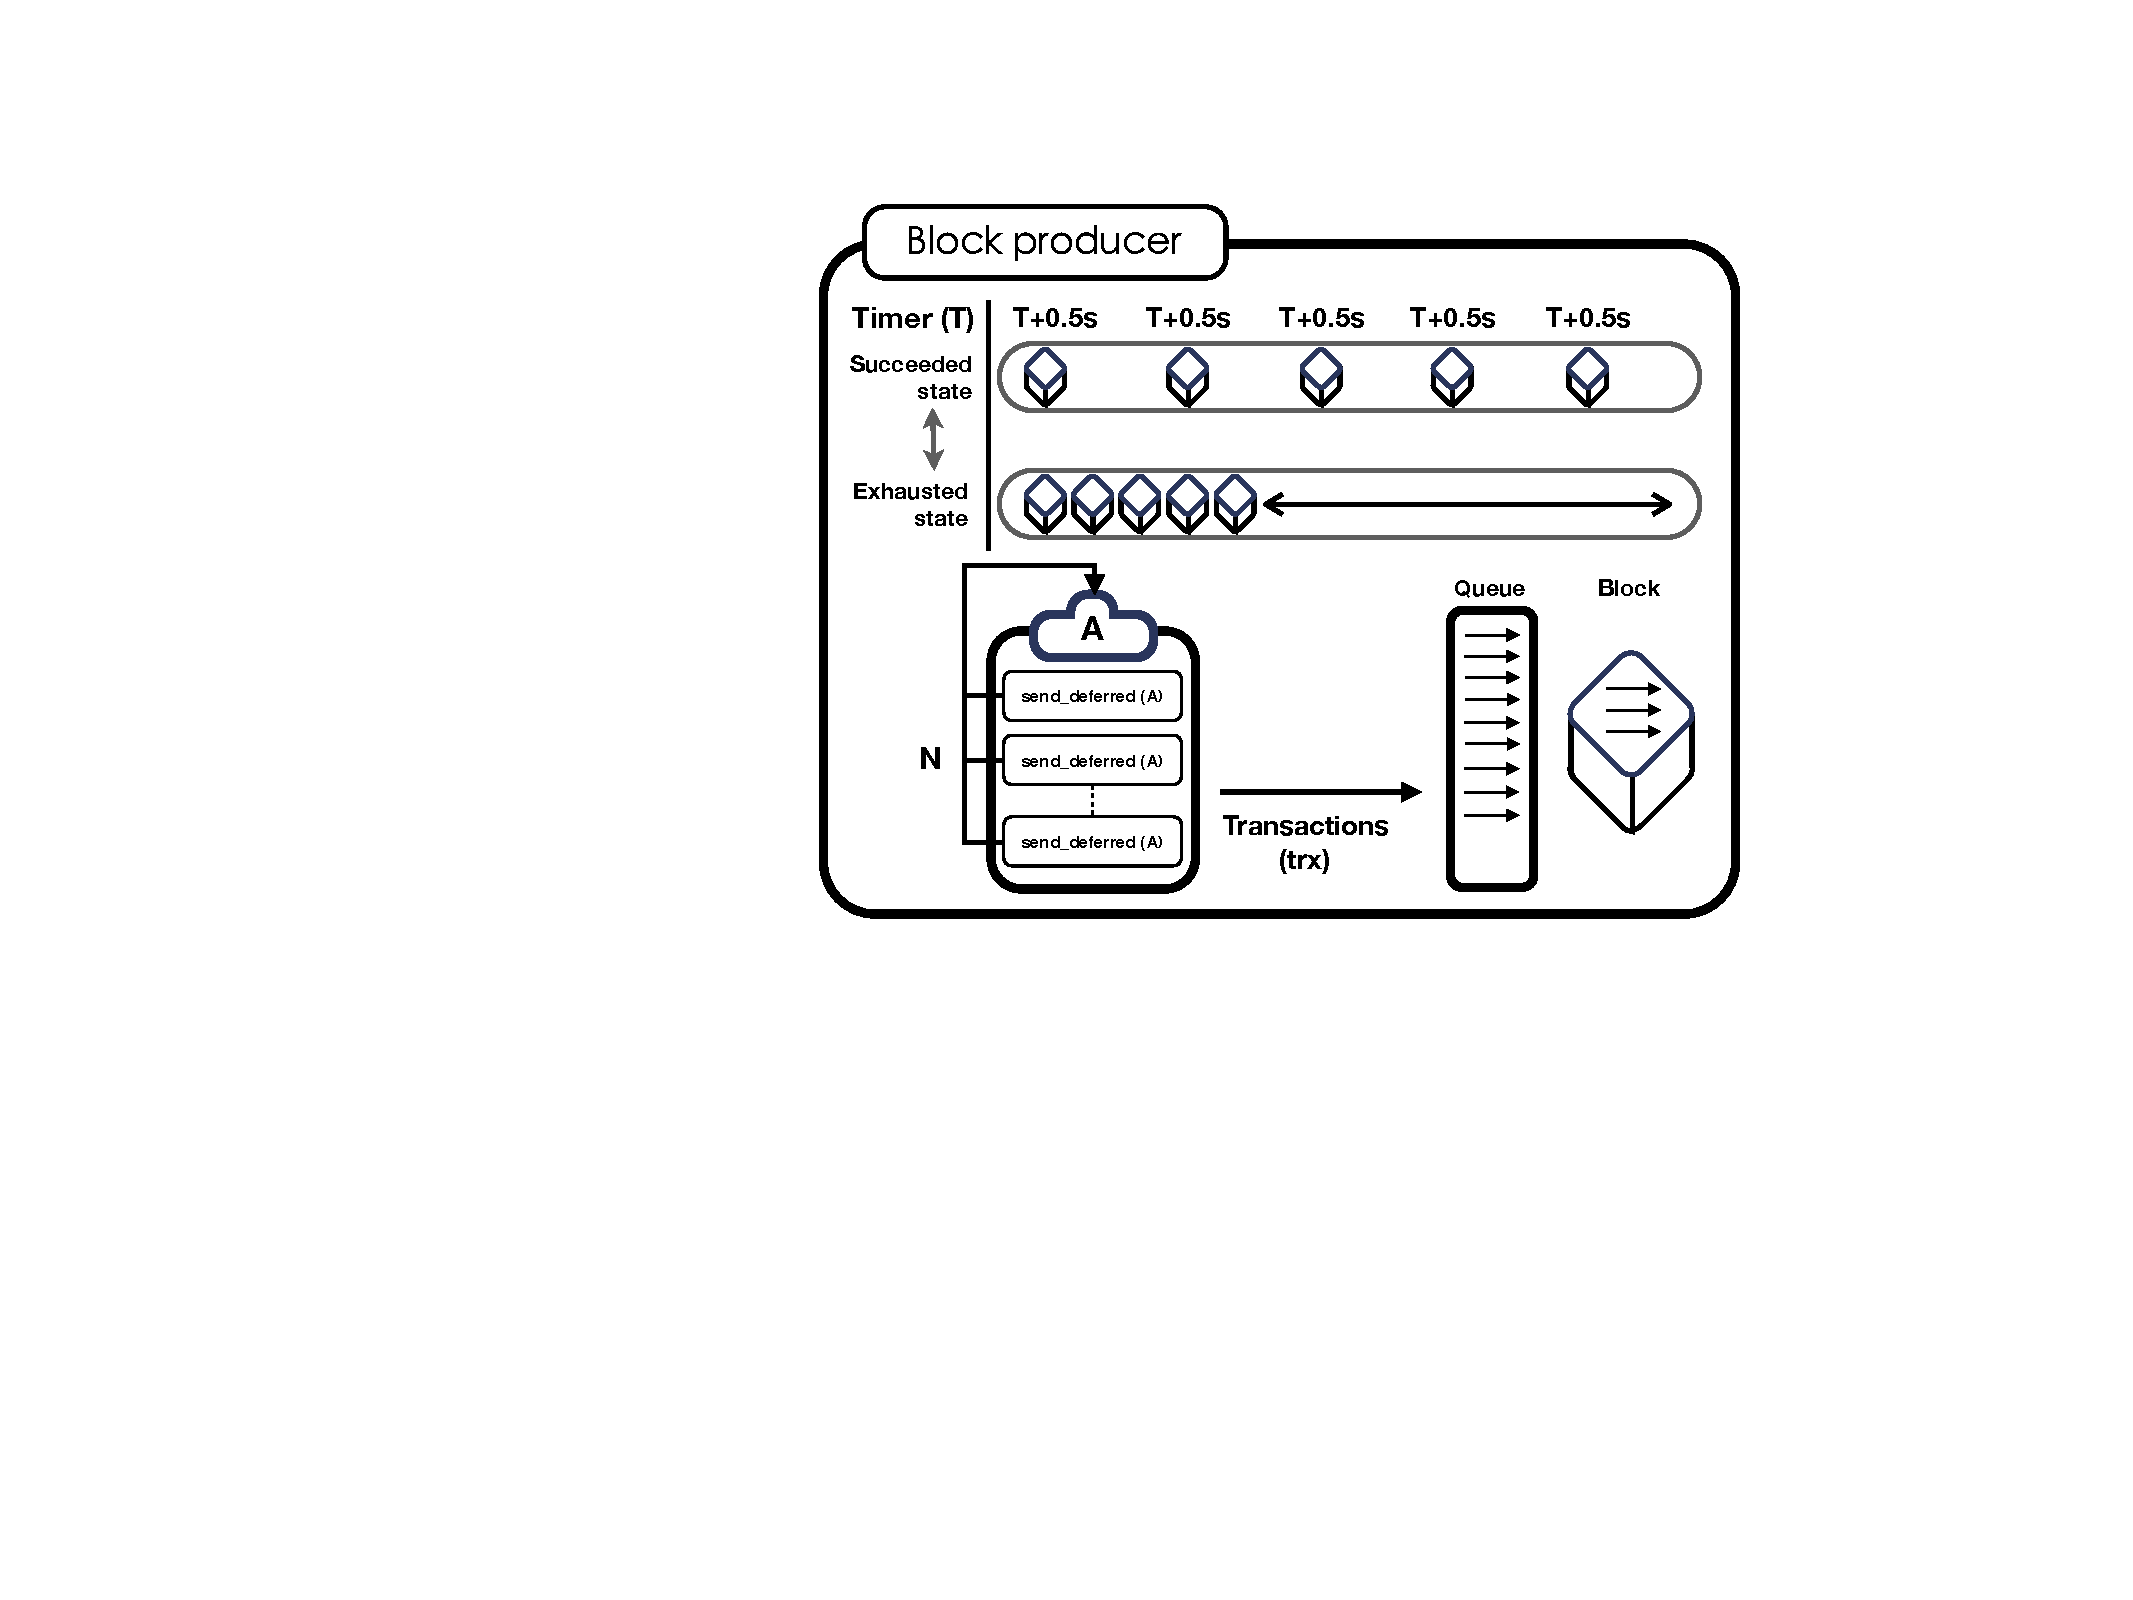
\includegraphics[width=0.9\linewidth]{figures/BlockDOS.pdf}
  \caption{Overview of the \NODEDOS attack.}
  \label{fig:pow}
\end{figure}

\PP{Block generation procedures.}
The \eos system has two internal policies; 1) a \BP should generate a block
within every 0.5 seconds; 2) a \BP limits its resource usage for processing
transactions within a block. Specifically, \eos limits the execution time as
well as the amount of \cpu and \net for processing transactions within a single
block.

To enforce these block generation policies, \eos has four internal states,
including \textit{succeeded} and \textit{exhausted} states. We only explain
these two states relevant to initiate the \NODEDOS attack.
%
In the succeeded state, a \BP generates a block for every 0.5 seconds. When a
\BP completes given transactions earlier than 0.5 seconds, it waits further and
then propagates the resulting block to other \BPs.
%
If the resource usage for processing transactions within a block is over a
specified threshold, it switches its state to the exhausted state and generates
as many blocks as possible without any waiting time to maximize its computation
resources.

A block generation delay arises when the exhausted state is changed back to the
succeeded state after a large number of blocks are generated in the exhausted
state. This delay stems from the time gap between the timestamp specified in a
block and the actual time when the block is generated. For each block, \eos
specifies a timestamp with the multiplication of the fixed time interval (0.5
seconds) with the number of all generated blocks in the entire \eos system that
precede the current block. That is, a \BP in the exhausted state could create a
block of which timestamp indicates a future time, when the \BP creates more than
one block within 0.5 seconds.
%
When the state is changed back to the succeeded state, the \BP attempts to
generate a new block with a future timestamp. It then pauses its block
generation until the real time matches the timestamp of this new block.


\PP{Attack conditions.}
In order to intentionally invoke such a block generation delay, the attack
should 1) change the succeeded state to the exhausted state, 2) make the \BP to
generate a large amount of blocks in the exhausted state, and then 3) change the
\BP back to the succeeded state.

By carefully analyzing the \eos system, we found that an adversary could easily
conduct the \NODEDOS attack by abusing two \eos features:
deferred transactions, and smart contract updates.

In general, a \BP executes a requested transaction right away, however, a
deferred transaction is scheduled later for its execution~\cite{EOSWHITEPAPER}.
The original purpose is to move computations into different shards or to create
a long-running process for continuance transactions.
%
To initiate a deferred transaction, an \SC invokes \texttt{send\_deferred()},
which makes a new asynchronous transaction on a \BP. Suppose an adversary
implements a malicious \SC that recursively invokes multiple deferred
transactions of itself. The execution of this \SC causes an exponentially
increasing number of crafted transactions, as~\autoref{fig:pow} illustrates.

When a \BP receives such a large number of transactions, its resources
eventually runs out and the \BP changes its state to the exhausted state.

After producing numerous transactions, an adversary changes the crafted \SC to a
totally different one. This change renders all the queued transactions from the
original \SC invalid because those transactions still attempt to call methods in
the original \SC which no longer exists.
%
Therefore, the \BP in the exhausted state marks the spurious transactions as
invalid and immediately process them, thereby generating a large amount of
blocks.
%
Consequently, these spurious blocks generates a huge gap between the timestamp
of the last block and the real time. When the \BP comes back to the succeeded
state, the \BP pauses its further block generation.
%
Consider that a \BP generates each one of 100 blocks for 0.2 seconds in the
exhausted state, thus taking 20 seconds ($0.2 * 100$). The timestamp of the last
block must be set to 50 seconds ($0.5 * 100$), thereby producing the time gap of
30 seconds. As a result, the \BP should delay its next block generation for 30
seconds when the state changes back to the succeeded one.
%
As the adversary is able to manage the number of blocks with the deferred
transaction, she can impose an arbitrary delay time, resulting in the DoS of
the \BP under the attack.



\begin{table}[!t]
\centering
\setlength\tabcolsep{0.07cm}
\caption{Estimated financial loss by the \NODEDOS attack}
\label{tab:nodedos_eval}

\begin{threeparttable}
\begin{tabular}{@{}rrcccrccr@{}}
\toprule

\multirow{2}[6]{*}{\textbf{\begin{tabular}[c]{@{}c@{}} Block \\ Count \end{tabular}}} &
&
\multicolumn{4}{c}{\textbf{Attacker}} &
&
\multicolumn{2}{c}{\textbf{Victim}}
\\
\cmidrule{3-6}
\cmidrule{8-9}
&
&
\multicolumn{1}{c}{\begin{tabular}[c]{@{}c@{}} Time\tnote{$\dagger$} \\ (min)\end{tabular}} &
\multicolumn{1}{c}{\begin{tabular}[c]{@{}c@{}} \cpu \\ (min)\end{tabular}} &
\multicolumn{1}{c}{\begin{tabular}[c]{@{}c@{}} \net \\ (MiB)\end{tabular}} &
\multicolumn{1}{c}{\begin{tabular}[c]{@{}c@{}} Cost\tnote{$\ddagger$} \\ (EOS)\end{tabular}} &
&
\multicolumn{1}{c}{\begin{tabular}[c]{@{}c@{}} Delay \\ (min)\end{tabular}} &
\multicolumn{1}{c}{\begin{tabular}[c]{@{}c@{}} Loss\tnote{$\ast$} \\ (EOS)\end{tabular}}
\\
\midrule
376   &  & 0.92    & 1.23  & 16.13   & 480   &  & 2.05 & 40,802  \\
704   &  & 2.06    & 2.32  & 34.72   & 910   &  & 3.56 & 70,856  \\
1,106 &  & 3.02    & 3.65  & 50.82   & 1,426  &  & 5.67 & 112,851  \\
1,471 &  & 4.00    & 4.85  & 65.53   & 1,894  &  & 7.46 & 148,478  \\
1,840 &  & 5.04    & 6.07  & 79.69   & 2,368  &  & 9.12 & 181,518 \\
\bottomrule
\end{tabular}

\footnotesize
\begin{tablenotes}
\item [$\ast$] We estimated the loss of \eos from the total volume of traded EOS
    tokens in April 2019.
\item [$\dagger$] As this attack creates a large number of transactions, it was
    difficult to precisely control the attack duration.
\item [$\ddagger$] The attack cost is estimated by multiplying the total staked
    EOS tokens by the ratio of the used \cpu and \net to their total capacity.
\end{tablenotes}
\end{threeparttable}
\end{table}


We conducted experiments to measure the extent of the losses that this attack
can cause to the \eos system.
%
We created a malicious \SC that internally makes six deferred transactions
that invoke the \SC itself, thus causing every single transaction to invoke the
execution of the same \SC six times.

\autoref{tab:nodedos_eval} summarizes the experimental results.
%
The block count describes the total number of blocks created during the attack.
%
The \textit{Attacker} columns describe the time and \eos resources consumed
during the attack.
%
%The \textit{Cost} column represents required EOS tokens during the attack.
%
Note that the exact number of required EOS tokens can vary depending on the
total number of staked EOS tokens (see~\S\ref{ss:stake}). Here, we calculated
them using the required values of \cpu and \ram in the real \eos system at the
time of the submission.
%
However, since the EOS tokens are returned after unstaking \cpu and \net as
described in~\S\ref{ss:stake}, the cost of the attack can be considered as zero.
%
The \textit{Victim BP} columns show the time delay of the BPs and the expected
number of EOS tokens that are not traded due to the corresponding delay,
respectively.
%
We estimated the loss based on the number of actual EOS tokens conducted in the
main \eos network. The equations for calculating the delay time ($T_{delay}$)
and the estimated loss ($E_{loss}$) are shown as below:

\begin{equation*}
\begin{gathered}
    E_{min} = E_{April} / ((60\ mins)*(24\ hrs)*(30\ days))
    \\
    T_{delay} = (T_{limit}*N_{blocks})-\sum_{i=1}^{N_{blocks}} T_{block_{i}}
    \\
    E_{loss} = E_{min} * T_{delay}
\end{gathered}
\end{equation*}

$E_{April}$ represents the number of EOS tokens actually signed in April 2019,
which was 859,821,765, and $E_{min}$ represents its one-minute average;
$T_{limit}$ is the time limit for executing each transaction in \eos, which is
0.5 seconds; $N_{blocks}$ is the number of blocks created, and $T_{block_{i}}$
is the execution time of i-th block during the attack.

The consequences of the attack are severe since a single adversary running the
attack for 5 minutes with 2,368 EOS tokens causes a financial loss of
181,518 EOS as well as undermines the service availability for nine
minutes.
%
Note that the cost of the attack is zero since the resource of the adversary
spent for the attack is returned in the very next day. In addition, coordinated
attacks targeting many SCs can certainly cause the DoS at all BPs. We reported
this bug to the \PLATFORM foundation, and they marked it as one of the most
critical bugs.

The \eos developers patched this bug by adding a timestamp check for each \eos
block generation. This patch makes a \BP to compute the expected time for a
newly generated block and checks whether the difference between this expected
time and the real time is within 0.5 seconds. If so, the \BP generates the next
block without any delays. Otherwise, it waits until the real time reaches the
expected time. This check prevents a block generated in the exhausted state from
having a future timestamp.






\section{DoS by draining EOS resources}
This section presents two DoS attacks: \TESER and \SCPDOS attacks. Both attacks
aim to undermine the service availability of a target \SCP by draining staked
\cpu and \ram, respectively.

\subsection{\TESER attack}
\label{label_teser}




\begin{table}[!t]
    \caption{The amount of \cpu and \ram consumed in the \TESER attack}
\label{tab:TeserResult}
\centering
\setlength\tabcolsep{0.1cm}

%\begin{threeparttable}
\begin{tabular}{@{}rcccccc@{}}
\toprule

\multirow{2}[5]{*}{\textbf{\begin{tabular}[c]{@{}c@{}} Attack \\ Count \end{tabular}}}&
&
\multicolumn{2}{c}{\textbf{Attacker}} &
&
\multicolumn{2}{c}{\textbf{Victim \SCP}} \\
\cmidrule{3-4}
\cmidrule{6-7}
&
&
\begin{tabular}[c]{@{}c@{}}\net \\ (KiB)\end{tabular} &
\begin{tabular}[c]{@{}c@{}}\cpu \\ (ms)\end{tabular} &
&
\begin{tabular}[c]{@{}c@{}}\net \\ (KiB)\end{tabular} &
\begin{tabular}[c]{@{}c@{}}\cpu \\ (ms)\end{tabular} \\ \midrule
1   & & 0.137 & 0.146 & & 3.562 & 0.400 \\
10  & & 1.329 & 1.485 & & 3.555 & 4.336 \\
20  & & 2.655 & 2.938 & & 3.549 & 8.352 \\
30  & & 3.980 & 4.474 & & 3.544 & 12.53 \\
50  & & 6.626 & 7.422 & & 3.534 & 20.74 \\
100 & & 13.21 & 15.23 & & 3.509 & 41.19 \\
\bottomrule
\end{tabular}

\end{table}


We present a novel attack that depletes all the \cpu staked for the execution of
a target \SC, thus making this \SC unavailable for further execution. The goal
of the adversary is to render the target \SC unavailable for any \BP by
depleting  all the \cpu staked by the \SC owner in exchange for the \cpu staked
by the adversary. We refer to this attack as an \textit{\TESER} attack.

An \SC often invokes \texttt{send\_deferred()} that generates a deferred
transaction for the execution of another \SC. By design, this execution of an
\SC requires \cpu from 1) the user who initiated the transaction or 2) the \SCP
of the original \SC.
%
However, spending \cpu belonging to a user requires the consent of this user
that grants the \code permission~\cite{EOSWHITEPAPER} to the \SC. Because this
permission is so sensitive that it allows the \SC to manage the EOS tokens of
the user, \users are naturally hesitant to grant this permission.
%
Therefore, \SCPs often use their staked \cpu for deferred transactions to
facilitate the wide adoption of their \SCs.

When the staked \cpu of an \SCP is exhausted, the corresponding \SC becomes
unavailable for 24 hours.

The \TESER attack exploits this feature, by continuously consuming the \cpu of
the victim \SCP. As a result, the attack is cost-effective if the total use of
the staked \cpu of the victim \SCP is greater than that of the adversary. The
adversary could also speed up the attack by creating an SC that recursively
calls itself as well as the target SC similar to the \NODEDOS attack.

To demonstrate the tangible threat of the \TESER attack, we sampled one of the
vulnerable \SCs~\footnote{We intentionally omitted the SC name in the \TESER
attack.} among the SCs that we collected from the main \eos network. In order
to do this, we manually analyzed a few SCs to check if a
\texttt{send\_deferred()} function call exists at the beginning of the SC
without a proper user validation.

\autoref{tab:TeserResult} shows the experimental results. During the experiment,
we varied the number of calling the target SC from 1 to 100.

When we conducted the attack once, the consumed \cpu of the victim SCP (11.50
ms) reached almost three times as much as that of the adversary (4.136 ms). The
gap in \cpu between the attacker and the victim \SCP increases almost at an
almost constant rate.
%increases as $N_{APB}$
This result demonstrates the feasibility of the \TESER attack that an adversary
can intentionally dry off the victim using only a small \cpu amount.




\subsection{\SCPDOS attack}
\label{SCPDOS}


% Attack summary
We present another threat that allows an adversary to deplete the \ram of a
victim \SCP by inserting spurious data, which results in the DoS for the \SCP.
%This attack targets the \ram of an \SCP with vulnerable \SC code, and
We refer to this attack as an \textit{\SCPDOS} attack.

Compared to other blockchain systems, \ram is another unique component of \eos
that abstracts the available data storage for executing an SC. Unlike \cpu,
\SCPs are able to choose either themselves or other users who execute their \SCs
to pay for the cost of storing user data without any permission.

In addition, \eos stores data in the form of a key-value pair, as in general
database systems. Thus, it is recommended that one should properly create a
unique key for each data insertion to prevent storing duplicated data.
%
When an \SCP chooses to pay for his/her SC instead of the user without such
consideration, his/her \SC can become vulnerable.

That is, an adversary can keep storing spurious data to \ram by exploiting this
vulnerable \SC until there is no remaining \ram purchased by the \SCP, which
eventually causes the DoS of the vulnerable \SC.

Among the collected SCs, we manually searched ones that use the \ram of \SCPs
and implement no measure to prevent the same user from storing unlimited data.
We experimented one vulnerable \SC~\footnote{We intentionally omitted the SC
name in the \SCPDOS attack.} as a case study to show the feasibility of the
\SCPDOS attack.
%\texttt{danakilblock} and used this \SC for
%our experiment.
%

\begin{figure}[!t] %%%2 t->h or ht
\centering
  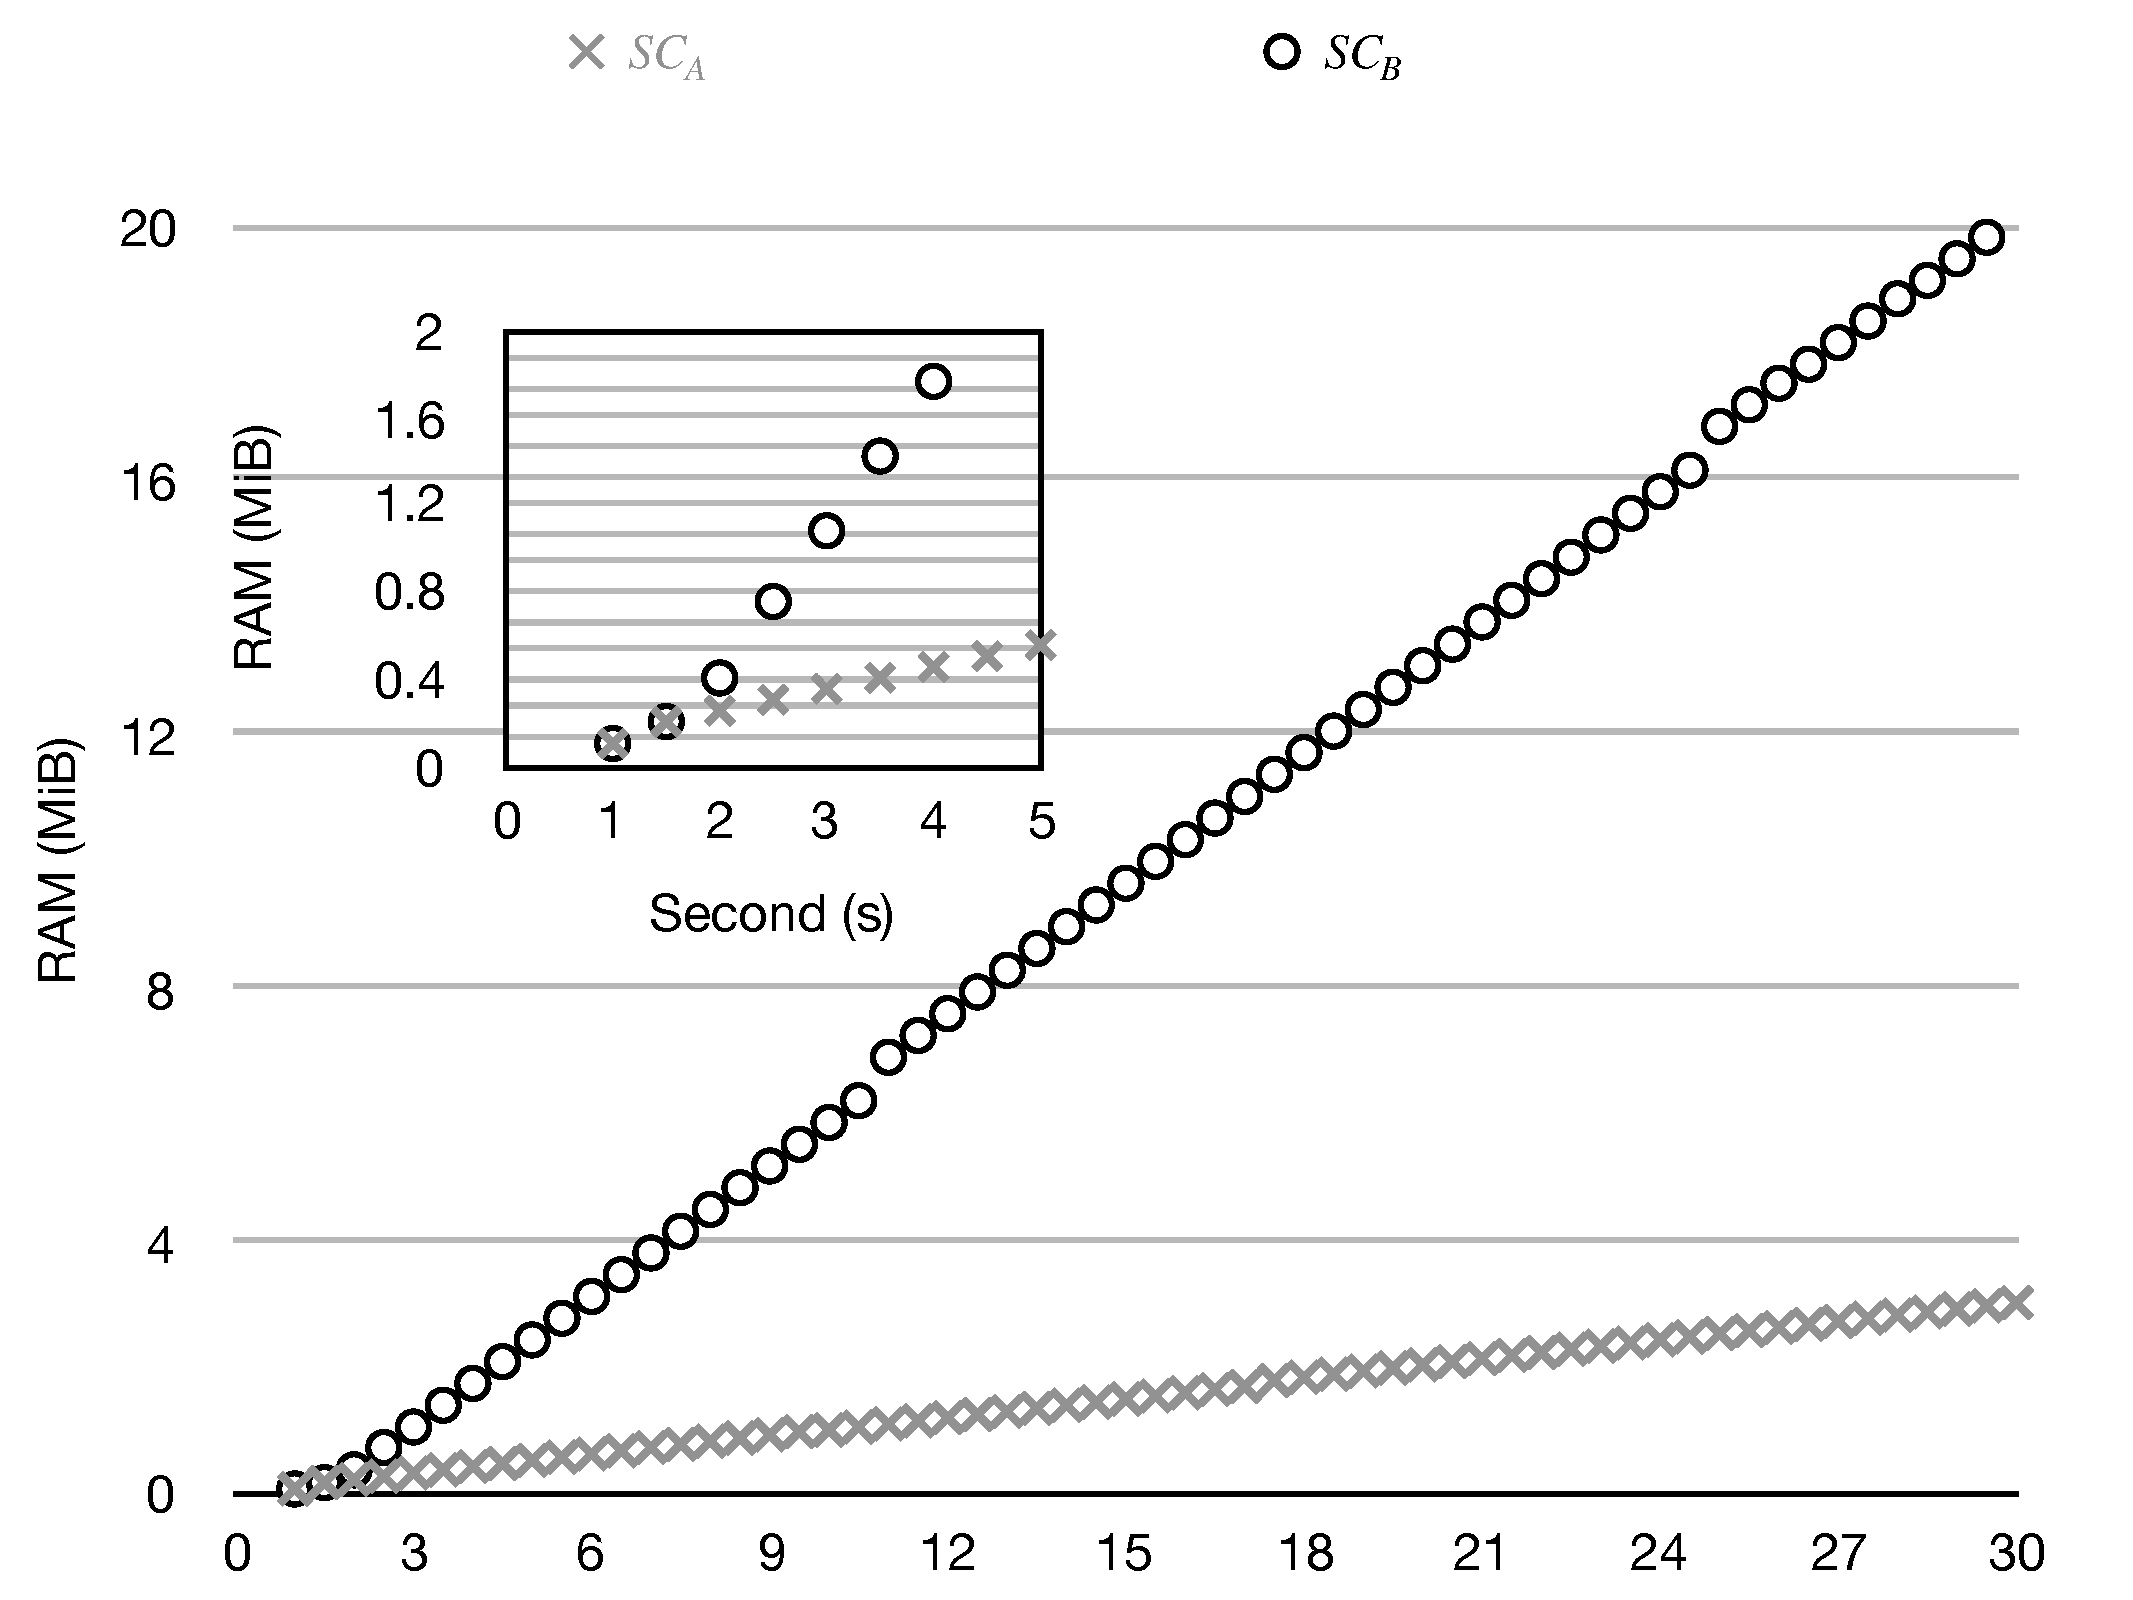
\includegraphics[width=0.8\linewidth]{figures/CREAT2.pdf}
  \caption{The amount of \ram consumed by the \SCPDOS attack.}
  %(Target SC: \texttt{danakilbock})
  \label{fig:scpdos}
\end{figure}


To conduct the attack, we implemented two additional SCs and compared their
efficacy.
%
$SC_{A}$ sends the vulnerable \SC a transaction that stores spurious data at the
\ram staked by the \SCP of the \SC. It then invokes itself via one
\texttt{send\_deferred()} call. $SC_{B}$ does the same as $SC_{A}$, however, it
invokes \texttt{send\_deferred()} twice, thus executing two instances of the \SC
at once.

\autoref{fig:scpdos} shows the experimental results. As the graph shows, the
slope of $SC_{B}$ is much steeper than that of $SC_{A}$. It only took 30 seconds
to deplete 20 MB for $SC_{B}$.
%
The actual efficacy of the \SCPDOS attack can differ depending on how much
of \ram is consumed and how the execution logic is implemented; however, this is
only a matter of time.

Once the \ram of the attacked \SCP is exhausted, the function for the \SC to use
\ram becomes no longer available.
%
Here, the \SCP can operate the \SC again by purchasing additional \ram; however,
this is only a temporary measure.
%
To sort out this problem, \SCPs should add a proper defense mechanism by
modifying the source code of the \SC and have to delete all the \ram tables
which may contain valuable user data.


\subsection{\TOCTOU attack}
\label{label_toctou}
\begin{figure}[!t] %%%1 t->h or ht
\centering
  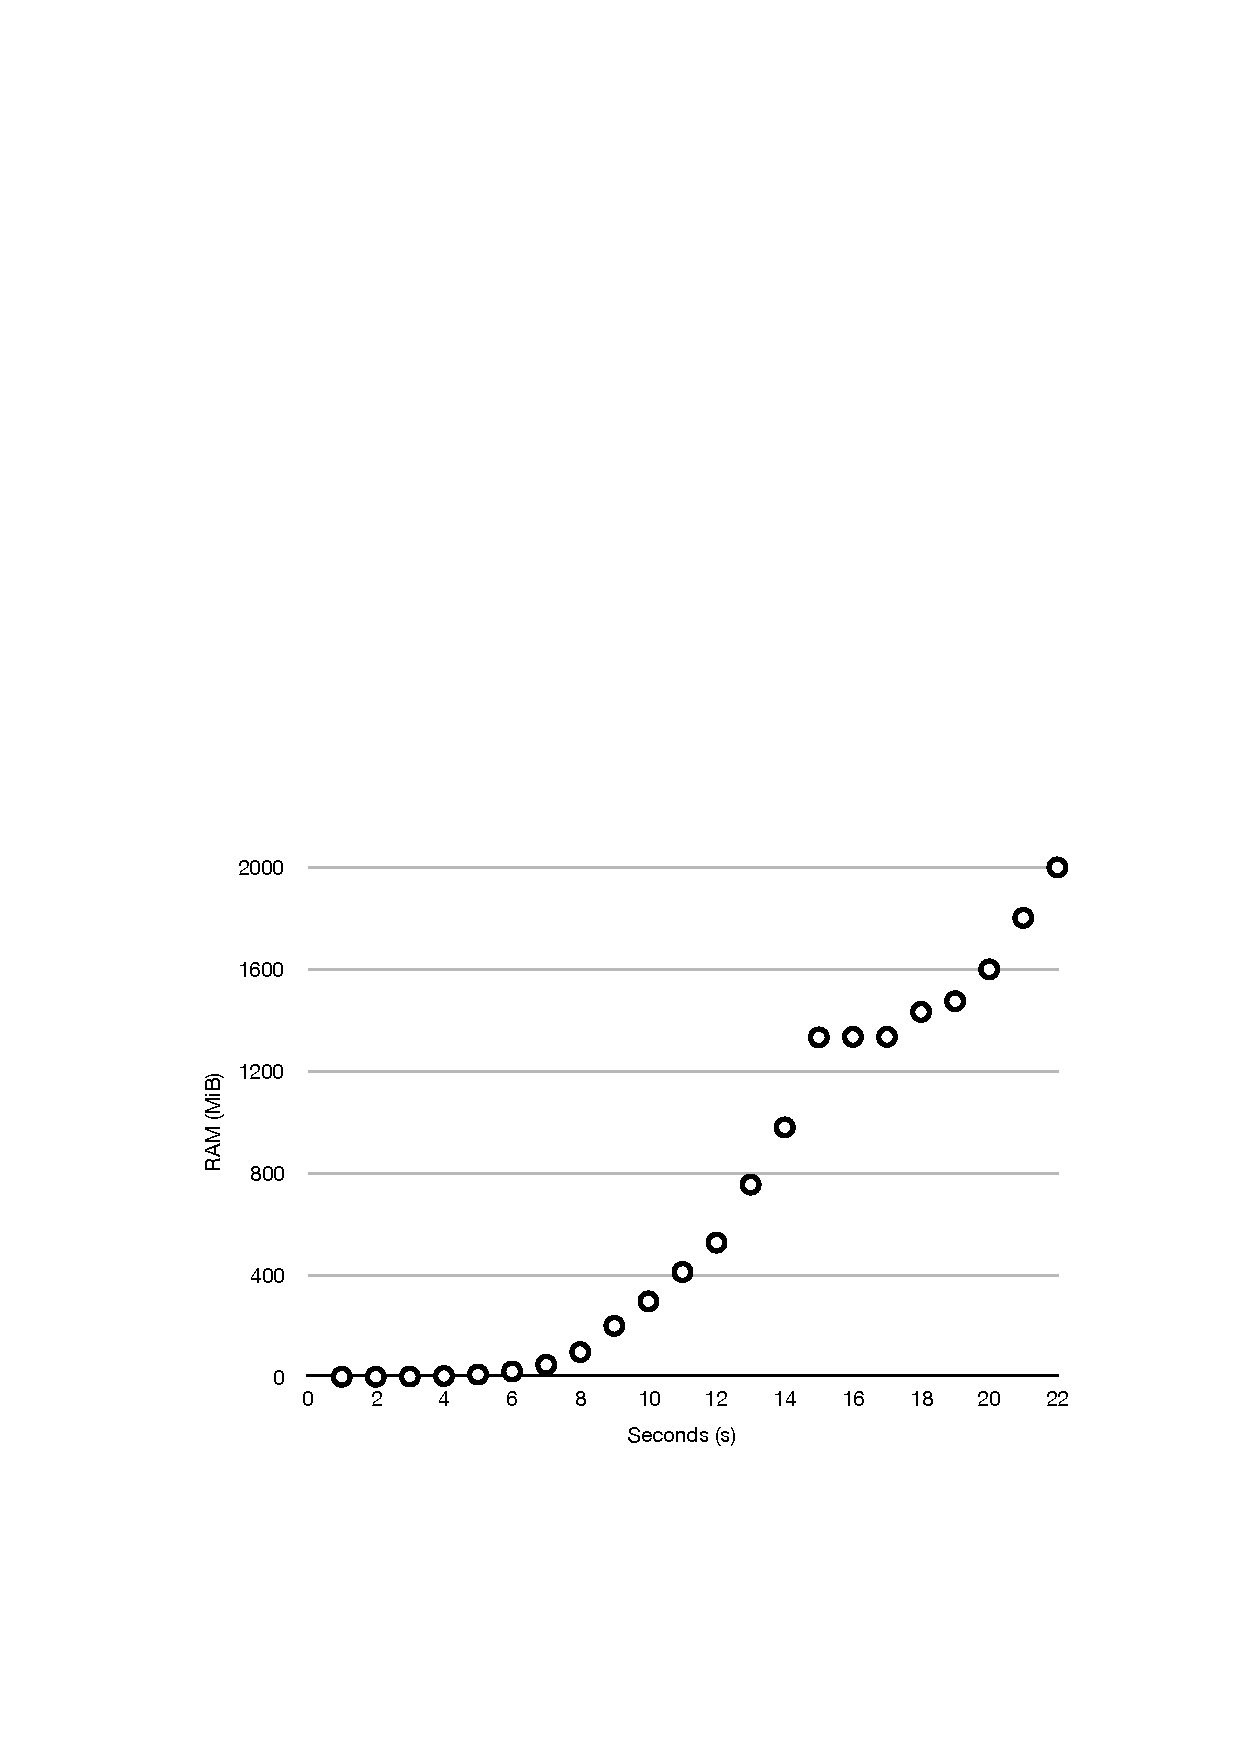
\includegraphics[width=0.8\linewidth]{figures/RAMSOMWARE_EVAL.pdf}
  \caption{The estimated \ram loss by the \TOCTOU attack.}
  \label{fig:toctou}
\end{figure}

% How attack works?`
We present the \textit{\TOCTOU} attack, a new threat that enables the adversary
to take possession of the resources of victims including \EOS tokens, \cpu, and
\ram, leveraging misplaced trust in \SCs. This attack takes advantage of the
fact that the SC of the adversary for executions can be different from the \SC
for which a victim granted the \code permission for privileged operations. This
is a classic time-of-check to time-of-use (TOCTOU) attack.

The adversary begins the attack by uploading a benign \SC. This benign \SC
requests the eosio.code permission from users for further execution.
%
As described in~\S\ref{ss:receiver}, users do not want to grant their permission
to SCPs in general.
%
In order to get the \code permission, the adversary can publish the source code
of the benign SC and obtain a safety inspection; there exist third-party
services that test the security of the submitted SCs~\cite{eospark}.
%
The adversary then promotes this benign \SC on his/her own website along with
the safety inspection results. A victim checks the published code as well as the
inspection results and decides to grant the permission to this \SC.
%
Later, the adversary switches the \SC to a malicious one, but the victim does
not recognize this change.
%
Thus, the victim is highly likely to run this changed \SC.
%
However, the \PLATFORM system does not warn or notify the victim of any code
changes made by the adversary.
%
This attack stems from the design decision of \PLATFORM that allows an \SCP to
update and revise their \SC without notifying users of such \SC changes.

One attack scenario is to lock the \ram of victims for ransom. Assuming that the
adversary is capable of obtaining the \code permission from victims, the attack
\SC can call itself repeatedly via \texttt{send\_deferred()} while storing
spurious data using the \ram of the victim until they are completely exhausted.
Unlike \cpu or \net which are restored every 24 hours, the \ram will be locked
until the adversary releases their usage. Therefore, the adversary can ask a
ransom in exchange for returning the locked \ram.

We conducted an experiment to check the feasibility of this attack in our
testing environment. We prepared a ransomware \SC and a victim account that
grants the \code permission to this \SC.
%
To fasten the completion of \ram exhaustion, we used the same methodology
described in~\S\ref{label_reentrancy-attack}, whereby the attack \SC recursively
invokes \texttt{send\_deferred()} multiple times. As~\autoref{fig:toctou} shows,
it took only around 22 seconds to deplete 2 GB of \ram, which is the \ram
capacity of the user with the most \ram when excluding the \eos
foundation~\cite{eospark}.



